%========================================
% LESSON CONTENT: Desigualdades Lineales
%========================================

\lesson{Desigualdades Lineales}

En esta lección introducimos las desigualdades lineales en una variable, sus reglas de manipulación, la resolución paso a paso y la representación del conjunto solución con notación de intervalos y en la recta real. También vemos desigualdades compuestas del tipo ``y'' (intersección) y ``o'' (unión), y practicamos con ejercicios.

\subsectiontitle{Conceptos básicos}

\begin{definition}
Una \textbf{desigualdad} es una expresión matemática que compara dos cantidades usando los símbolos:
\begin{itemize}
    \item $<$ (menor que)
    \item $>$ (mayor que)
    \item $\le$ (menor o igual que)
    \item $\ge$ (mayor o igual que)
\end{itemize}

Una \textbf{solución} de una desigualdad es todo valor de la variable que hace verdadera la desigualdad.

El \textbf{conjunto solución} de una desigualdad generalmente es un intervalo o unión de intervalos en $\mathbb{R}$.
\end{definition}

\begin{example}
\textbf{Diferencia entre ecuación y desigualdad:}

\begin{itemize}
    \item \textbf{Ecuación:} $4x - 7 = 19$ tiene solución única $x = \dfrac{26}{4} = \dfrac{13}{2}$.

    \item \textbf{Desigualdad:} $4x - 7 \le 19$ tiene soluciones $x \le \dfrac{26}{4} = \dfrac{13}{2}$, que es un intervalo $\left(-\infty, \dfrac{13}{2}\right]$.
\end{itemize}

\textbf{Representación gráfica:}

\begin{center}
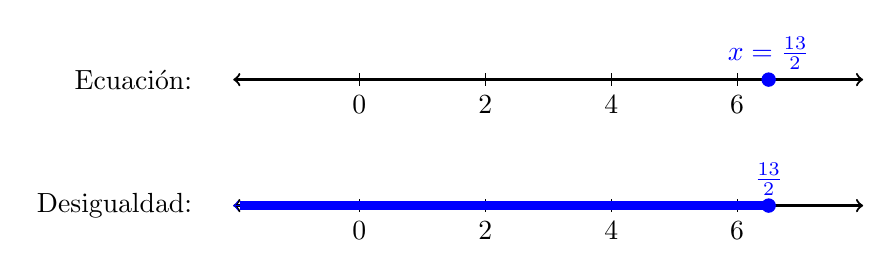
\begin{tikzpicture}[scale=0.8]
    % Equation solution (single point)
    \draw[thick, <->] (-2,2) -- (8,2);
    \foreach \x in {0,2,4,6}
        \draw (\x,2.1) -- (\x,1.9) node[below] {\x};
    \node at (-2.5,2) [left] {Ecuación:};
    \filldraw[blue] (6.5,2) circle (3pt) node[above] {$x = \frac{13}{2}$};

    % Inequality solution (interval)
    \draw[thick, <->] (-2,0) -- (8,0);
    \foreach \x in {0,2,4,6}
        \draw (\x,0.1) -- (\x,-0.1) node[below] {\x};
    \node at (-2.5,0) [left] {Desigualdad:};
    \draw[blue, line width=3pt] (-1.9,0) -- (6.5,0);
    \filldraw[blue] (6.5,0) circle (3pt) node[above] {$\frac{13}{2}$};
    \draw[blue, <-] (-2,0) -- (-1.5,0);
\end{tikzpicture}
\end{center}

\vspace{0.3cm}
\textbf{Notación de intervalos:}

La solución $x \le \dfrac{13}{2}$ se escribe en notación de intervalos como $\left(-\infty, \dfrac{13}{2}\right]$.

\begin{itemize}
    \item Paréntesis ( o ) indica que el extremo \textbf{no está incluido} (desigualdad estricta: $<$ o $>$)
    \item Corchete [ o ] indica que el extremo \textbf{está incluido} (desigualdad no estricta: $\le$ o $\ge$)
    \item El infinito ($\infty$ o $-\infty$) siempre lleva paréntesis
\end{itemize}

\textbf{Tabla de referencia:}

\begin{center}
\begin{tabular}{|c|c|c|}
\hline
\textbf{Desigualdad} & \textbf{Notación de intervalos} & \textbf{Representación gráfica} \\
\hline
$x < a$ & $(-\infty, a)$ & 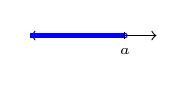
\begin{tikzpicture}[scale=0.4, baseline=0.1cm]
    \draw[<->] (-2,0) -- (2,0);
    \draw[blue, line width=2pt] (-2,0) -- (1,0);
    \draw[blue] (1,0) circle (2pt);
    \filldraw (1,0.1) -- (1,-0.1) node[below] {\tiny $a$};
\end{tikzpicture} \\
\hline
$x \le a$ & $(-\infty, a]$ & 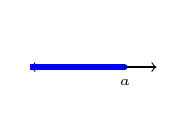
\begin{tikzpicture}[scale=0.4, baseline=0.5cm]
    \draw[<->] (-2,0) -- (2,0);
    \draw[blue, line width=2pt] (-2,0) -- (1,0);
    \filldraw[blue] (1,0) circle (2pt);
    \filldraw (1,0.1) -- (1,-0.1) node[below] {\tiny $a$};
\end{tikzpicture} \\
\hline
$x > a$ & $(a, \infty)$ & 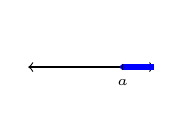
\begin{tikzpicture}[scale=0.4, baseline=0.5cm]
    \draw[<->] (-2,0) -- (2,0);
    \draw[blue, line width=2pt] (1,0) -- (2,0);
    \draw[blue] (1,0) circle (2pt);
    \filldraw (1,0.1) -- (1,-0.1) node[below] {\tiny $a$};
\end{tikzpicture} \\
\hline
$x \ge a$ & $[a, \infty)$ & 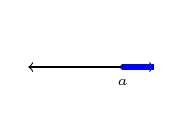
\begin{tikzpicture}[scale=0.4, baseline=0.5cm]
    \draw[<->] (-2,0) -- (2,0);
    \draw[blue, line width=2pt] (1,0) -- (2,0);
    \filldraw[blue] (1,0) circle (2pt);
    \filldraw (1,0.1) -- (1,-0.1) node[below] {\tiny $a$};
\end{tikzpicture} \\
\hline
$a < x < b$ & $(a, b)$ & 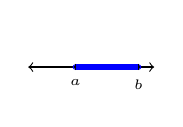
\begin{tikzpicture}[scale=0.4, baseline=0.5cm]
    \draw[<->] (-2,0) -- (2,0);
    \draw[blue, line width=2pt] (-0.5,0) -- (1.5,0);
    \draw[blue] (-0.5,0) circle (2pt);
    \draw[blue] (1.5,0) circle (2pt);
    \filldraw (-0.5,0.1) -- (-0.5,-0.1) node[below] {\tiny $a$};
    \filldraw (1.5,0.1) -- (1.5,-0.1) node[below] {\tiny $b$};
\end{tikzpicture} \\
\hline
\end{tabular}
\end{center}
\end{example}

\newpage

\subsectiontitle{Reglas para desigualdades}

\begin{theorem}
Sea $A, B, C \in \mathbb{R}$.

\textbf{Regla 1 (Suma):} Si $A \le B$, entonces $A + C \le B + C$.

\textbf{Regla 2 (Resta):} Si $A \le B$, entonces $A - C \le B - C$.

\textbf{Regla 3 (Multiplicación/División por positivo):} Si $C > 0$ y $A \le B$, entonces
\[CA \le CB \quad \text{y} \quad \dfrac{A}{C} \le \dfrac{B}{C}.\]

\textbf{Regla 4 (Multiplicación/División por negativo):} Si $C < 0$ y $A \le B$, entonces
\[CA \ge CB \quad \text{y} \quad \dfrac{A}{C} \ge \dfrac{B}{C}.\]

\footnotesize
\begin{center}
\textcolor{red}{\textbf{¡Se invierte la desigualdad!}}
\end{center}
\normalsize

\textbf{Regla 5 (Recíprocos positivos):} Si $0 < A \le B$, entonces
\[\dfrac{1}{A} \ge \dfrac{1}{B}.\]

\footnotesize
\begin{center}
	\textcolor{red}{\textbf{¡Se invierte la desigualdad!}}
\end{center}
\normalsize


\textbf{Regla 6 (Suma de desigualdades):} Si $A \le B$ y $C \le D$, entonces
\[A + C \le B + D.\]
\end{theorem}

\begin{warning}
\textbf{Punto clave:} Al multiplicar o dividir ambos lados de una desigualdad por un número negativo, se debe invertir la dirección de la desigualdad.

\textbf{Ejemplo:}
\begin{align*}
-2x &> 6 \\
x &< -3 \quad \text{(dividimos entre $-2 < 0$ e invertimos la desigualdad)}
\end{align*}

Este es el error más común al resolver desigualdades. ¡Tenga cuidado!
\end{warning}

\newpage

\subsectiontitle{Resolución de desigualdades lineales (una variable)}

La idea es aislar la variable aplicando las reglas anteriores, cuidando el cambio de sentido al multiplicar o dividir por números negativos.

\begin{example}
\textbf{Ejemplo 1: Desigualdad lineal sencilla}

Resuelva y grafique el conjunto solución de $4x - 7 \le 19$.

\solution
\begin{align*}
4x - 7 &\le 19 \\
4x &\le 26 \quad \text{(sumamos 7 a ambos lados)} \\
x &\le \dfrac{26}{4} \quad \text{(dividimos entre 4 > 0, sin cambiar el sentido)} \\
x &\le \dfrac{13}{2}
\end{align*}

\textbf{Solución en notación de intervalos:} $\left(-\infty, \dfrac{13}{2}\right]$

\textbf{Representación gráfica:}

\begin{center}
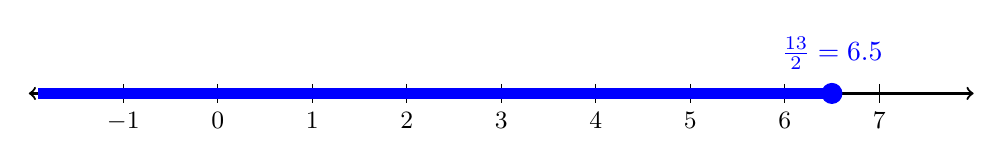
\begin{tikzpicture}[scale=1.2]
    \draw[thick, <->] (-2,0) -- (8,0);
    \foreach \x in {-1,0,1,2,3,4,5,6,7}
        \draw (\x,0.1) -- (\x,-0.1) node[below] {\small $\x$};

    % Solution: x <= 13/2 = 6.5
    \draw[blue, line width=4pt] (-1.9,0) -- (6.5,0);
    \filldraw[blue] (6.5,0) circle (3pt) node[above=5pt] {$\frac{13}{2} = 6.5$};

\end{tikzpicture}
\end{center}

\textbf{Interpretación:} El círculo relleno en $\dfrac{13}{2}$ indica que este valor está incluido en la solución ($\le$). La línea azul hacia la izquierda representa todos los números menores o iguales a $\dfrac{13}{2}$.
\end{example}

\newpage
\begin{example}
\textbf{Ejemplo 2: Desigualdad con coeficiente negativo}

Resuelva $-3x + 5 > 11$ y exprese en notación de intervalos.

\solution
\begin{align*}
-3x + 5 &> 11 \\
-3x &> 6 \quad \text{(restamos 5 de ambos lados)} \\
x &< -2 \quad \textcolor{red}{\textbf{(dividimos entre $-3 < 0$ e invertimos la desigualdad)}}
\end{align*}

\textbf{Solución en notación de intervalos:} $(-\infty, -2)$

\textbf{Representación gráfica:}

\begin{center}
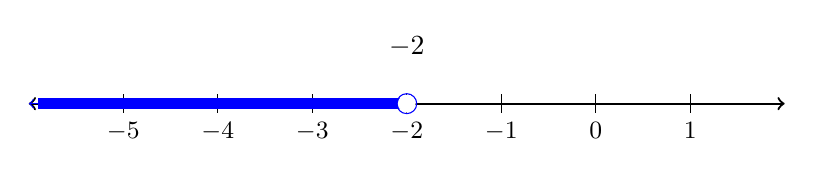
\begin{tikzpicture}[scale=1.2]
    \draw[thick, <->] (-6,0) -- (2,0);
    \foreach \x in {-5,-4,-3,-2,-1,0,1}
        \draw (\x,0.1) -- (\x,-0.1) node[below] {\small $\x$};

    % Solution: x < -2
    \draw[blue, line width=4pt] (-5.9,0) -- (-2,0);
    \draw[blue] (-2,0) circle (3pt);
    \filldraw[white] (-2,0) circle (2.5pt);
    \draw[blue, <-] (-6,0) -- (-5.5,0);
    \node at (-2,0.6) {$-2$};
\end{tikzpicture}
\end{center}

\textbf{Interpretación:} El círculo abierto en $-2$ indica que este valor \textbf{no está incluido} en la solución ($<$). La línea azul representa todos los números menores que $-2$.
\end{example}


\begin{example}
\textbf{Ejemplo 3: Desigualdad con fracciones}

Resuelva $\dfrac{2x - 3}{4} \ge \dfrac{x + 1}{2}$.

\solution

Multiplicamos ambos lados por 4 (que es positivo, por lo que no cambia el sentido):
\begin{align*}
\dfrac{2x - 3}{4} &\ge \dfrac{x + 1}{2} \\
4 \cdot \dfrac{2x - 3}{4} &\ge 4 \cdot \dfrac{x + 1}{2} \\
2x - 3 &\ge 2(x + 1) \\
2x - 3 &\ge 2x + 2 \\
-3 &\ge 2 \quad \text{(falso para todo $x$)}
\end{align*}

\textbf{Solución:} No hay solución. El conjunto solución es $\varnothing$ (conjunto vacío).

\textbf{Representación gráfica:} No hay puntos en la recta real que satisfagan la desigualdad.
\end{example}

\begin{example}
\textbf{Ejemplo 4: Multiplicación por número negativo}

Considere la desigualdad: $-6x + 4 < 0$

\solution
\begin{align*}
-6x + 4 &< 0 \\
-6x &< -4 \quad \text{(restamos 4)} \\
x &> \dfrac{-4}{-6} \quad \textcolor{red}{\textbf{(dividimos entre $-6 < 0$ e invertimos)}} \\
x &> \dfrac{2}{3}
\end{align*}

\textbf{Solución en notación de intervalos:} $\left(\dfrac{2}{3}, \infty\right)$

\textbf{Representación gráfica:}

\begin{center}
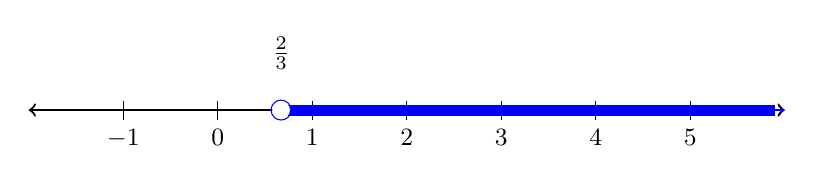
\begin{tikzpicture}[scale=1.2]
    \draw[thick, <->] (-2,0) -- (6,0);
    \foreach \x in {-1,0,1,2,3,4,5}
        \draw (\x,0.1) -- (\x,-0.1) node[below] {\small $\x$};

    % Solution: x > 2/3 ≈ 0.67
    \draw[blue, line width=4pt] (0.67,0) -- (5.9,0);
    \draw[blue] (0.67,0) circle (3pt);
    \filldraw[white] (0.67,0) circle (2.5pt);
    \draw[blue, ->] (5.5,0) -- (6,0);
    \node at (0.67,0.6) {$\frac{2}{3}$};
\end{tikzpicture}
\end{center}
\end{example}

\newpage

\subsectiontitle{Desigualdades compuestas}

Hay dos formas comunes de desigualdades compuestas:

\begin{definition}
\textbf{Tipo ``y'' (intersección):} $a < \text{expresión} \le b$

Se resuelve aplicando operaciones a los tres lados a la vez. La solución es la intersección de ambas condiciones.

\textbf{Tipo ``o'' (unión):} $\text{expresión} < a \;\;\text{o}\;\; \text{expresión} \ge b$

Se resuelve cada parte por separado y se toma la unión de las soluciones.
\end{definition}

\begin{example}
\textbf{Ejemplo 5: Desigualdad compuesta tipo ``y'' (intersección)}

Resuelva $4 \le 3x - 2 < 13$.

\solution

Aplicamos las operaciones a las tres partes:
\begin{align*}
4 &\le 3x - 2 < 13 \\
4 + 2 &\le 3x - 2 + 2 < 13 + 2 \quad \text{(sumamos 2 a las tres partes)} \\
6 &\le 3x < 15 \\
\dfrac{6}{3} &\le \dfrac{3x}{3} < \dfrac{15}{3} \quad \text{(dividimos entre 3 > 0)} \\
2 &\le x < 5
\end{align*}

\textbf{Solución en notación de intervalos:} $[2, 5)$

\textbf{Representación gráfica:}

\begin{center}
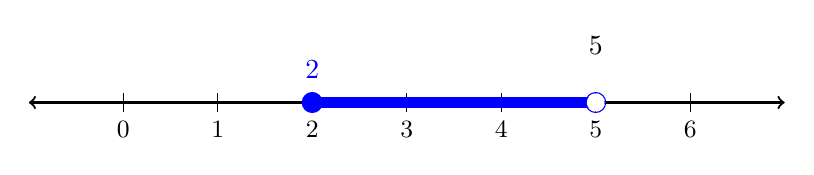
\begin{tikzpicture}[scale=1.2]
    \draw[thick, <->] (-1,0) -- (7,0);
    \foreach \x in {0,1,2,3,4,5,6}
        \draw (\x,0.1) -- (\x,-0.1) node[below] {\small $\x$};

    % Solution: 2 <= x < 5
    \draw[blue, line width=4pt] (2,0) -- (5,0);
    \filldraw[blue] (2,0) circle (3pt) node[above=5pt] {$2$};
    \draw[blue] (5,0) circle (3pt);
    \filldraw[white] (5,0) circle (2.5pt);
    \node at (5,0.6) {$5$};
\end{tikzpicture}
\end{center}

\textbf{Interpretación:} El círculo relleno en 2 indica que está incluido ($\le$). El círculo abierto en 5 indica que no está incluido ($<$).
\end{example}

\newpage

\begin{example}
\textbf{Ejemplo 6: Desigualdad compuesta tipo ``o'' (unión)}

Resuelva $2x + 1 < -3 \;\;\text{o}\;\; 2x + 1 \ge 7$.

\solution

Resolvemos cada desigualdad por separado:

\textbf{Primera parte:}
\begin{align*}
2x + 1 &< -3 \\
2x &< -4 \\
x &< -2
\end{align*}

\textbf{Segunda parte:}
\begin{align*}
2x + 1 &\ge 7 \\
2x &\ge 6 \\
x &\ge 3
\end{align*}

La solución es la \textbf{unión} de ambas: $x < -2$ \textbf{o} $x \ge 3$.

\textbf{Solución en notación de intervalos:} $(-\infty, -2) \cup [3, \infty)$

\textbf{Representación gráfica:}

\begin{center}
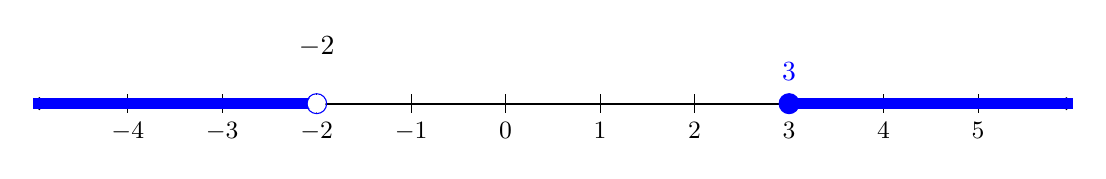
\begin{tikzpicture}[scale=1.2]
    \draw[thick, <->] (-5,0) -- (6,0);
    \foreach \x in {-4,-3,-2,-1,0,1,2,3,4,5}
        \draw (\x,0.1) -- (\x,-0.1) node[below] {\small $\x$};

    % Solution: x < -2 or x >= 3
    \draw[blue, line width=4pt] (-5,0) -- (-2,0);
    \draw[blue] (-2,0) circle (3pt);
    \filldraw[white] (-2,0) circle (2.5pt);
    \node at (-2,0.6) {$-2$};

    \draw[blue, line width=4pt] (3,0) -- (6,0);
    \filldraw[blue] (3,0) circle (3pt) node[above=5pt] {$3$};

    \draw[blue, <-] (-5,0) -- (-4.5,0);
    \draw[blue, ->] (5.5,0) -- (6,0);
\end{tikzpicture}
\end{center}

\textbf{Interpretación:} La solución consiste en dos regiones separadas: todos los números menores que $-2$ (círculo abierto) y todos los números mayores o iguales a 3 (círculo relleno).
\end{example}

\newpage

\subsectiontitle{Modelado con desigualdades}

Las desigualdades se usan para modelar situaciones donde hay restricciones o límites.

\begin{example}
\textbf{Ejemplo 7: Modelado con palabras}

Un boleto de cine y un refrigerio cuestan a lo más \$18. El refrigerio cuesta \$5. Si $x$ representa el costo del boleto, ¿qué valores de $x$ son posibles?

\solution

\textbf{Traducción:} ``a lo más \$18'' significa ``menor o igual que \$18''.

La desigualdad es:
\[x + 5 \le 18\]

Resolviendo:
\begin{align*}
x + 5 &\le 18 \\
x &\le 13
\end{align*}

\textbf{Solución:} El boleto puede costar a lo más \$13. En notación de intervalos: $(0, 13]$ (asumiendo que el precio debe ser positivo).

\textbf{Representación gráfica:}

\begin{center}
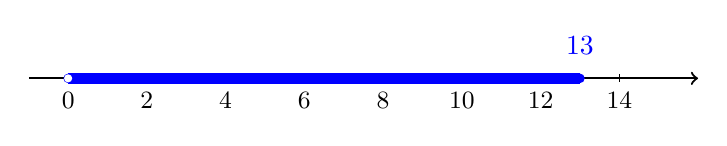
\begin{tikzpicture}[scale=0.5]
    \draw[thick, ->] (-1,0) -- (16,0);
    \foreach \x in {0,2,4,6,8,10,12,14}
        \draw (\x,0.1) -- (\x,-0.1) node[below] {\small $\x$};

    % Solution: 0 < x <= 13
    \draw[blue, line width=4pt] (0,0) -- (13,0);
    \draw[blue] (0,0) circle (3pt);
    \filldraw[white] (0,0) circle (2.5pt);
    \filldraw[blue] (13,0) circle (3pt) node[above=5pt] {$13$};
\end{tikzpicture}
\end{center}
\end{example}

\vspace{1cm}

\textbf{Palabras clave en problemas de desigualdades:}

\begin{center}
\begin{tabular}{|l|c|}
\hline
\textbf{Frase} & \textbf{Símbolo} \\
\hline
``a lo más'', ``como máximo'', ``no más de'' & $\le$ \\
``al menos'', ``como mínimo'', ``no menos de'' & $\ge$ \\
``más que'', ``mayor que'' & $>$ \\
``menos que'', ``menor que'' & $<$ \\
``entre $a$ y $b$'' (incluyendo ambos) & $a \le x \le b$ \\
``entre $a$ y $b$'' (sin incluir extremos) & $a < x < b$ \\
\hline
\end{tabular}
\end{center}
